\chapter{Specyfikacja zewnętrzna}
\label{ch:04}
\section{Wymagania sprzętowe i programowe}
Do działania aplikacji wymagany jest serwer, na którym uruchomiona będzie warstwa usługowa projektu. Bazując na przeprowadzonych testach wydajności działającej aplikacji można stwierdzić, że wykorzystanie zasobów jest niewielkie - średnio 300MB pamięci RAM, 60MB przestrzeni dyskowej oraz wykorzystanie procesora na poziomie 2\% (testy uruchamiane na procesorze Intel Core i5-8250U). Aplikacja wymaga stałego połączenia do Internetu aby poprawnie działać (komunikacja z zewnętrznym API Spotify) oraz urządzenie, na którym aplikacja będzie uruchomiona musi być kompatybilne z maszyną wirtualną Javy (JVM). Dodatkowo do uruchomienia oprogramowania wymagana jest Java w wersji co najmniej 21. Warstwa prezentacji także wymaga serwera HTTP, z którego pobierane będą potrzebne dla klienta pliki ze strukturą aplikacji oraz potrzebnymi skryptami. Dodatkowo system wymaga dostępu do silnika bazodanowego postgreSQL w wersji 16.1. Wszystkie elementy systemu mogą działać na jednym urządzeniu (serwer HTTP, API oraz bazy danych), bądź dowolnie rozłożone na kilka osobnych urządzeń.

Aby klient mógł korzystać z aplikacji wymagana jest przeglądarka internetowa na dowolnym urządzeniu wspierająca obsługę języka JavaScript, HTML5 oraz CSS3 oraz połączenie z serwerem.

\section{Sposób instalacji}
W celu instalacji należy pobrać skompilowane pliki projektu bądź skompilować je we własnym zakresie. Do kompilacji potrzebne będą następujące narzędzia: 
\begin{itemize}
\item Środowisko Java w wersji 21
\item Narzędzie Maven
\item Narzędzie wiersza poleceń Angular CLI (Command Line Interface)
\item Narzędzie Node Package Manager
\end{itemize}

Aby skompilować oprogramowanie warstwy usług należy uruchomić wiersz poleceń, odnaleźć plik pom.xml w plikach projektu i przejść do jego lokalizacji (folder "Backend"), a następnie wywołać następujące polecenie: 

\lstinline|mvn compile|


Warstwa interfejsu użytkownika kompilowana jest w analogiczny sposób. Należy uruchomić wiersz poleceń, odnaleźć ścieżkę projektu interfejsu użytkownika i przejść do głównego folderu (folder "Frontend"). Następnie należy wywołać polecenie

\lstinline|ng build|



\section{Sposób aktywacji}
Przed uruchomieniem systemu należy skonfigurować aplikację serwera. W folderze z projektem warstwy usług należy zlokalizować plik "application.properites", w którym znajdują się następujące właściwości, które należy ustawić:
\begin{itemize}
\item \lstinline|base.address| - adres serwera HTTP udostępniającego warstwę interfejsu użytkownika
\item \lstinline|qrcode.address.suffix| - przyrostek adresu, który zakodowany w formie kodu QR. Otrzymany adres w kodzie QR będzie złączeniem trzech elementów: adresu serwera HTTP (base.address), przyrostka (qrcode.address.suffix) oraz kodu dostępu do danej sesji.
\item \lstinline|spotify.authorize.callbackUrl.suffix| - przyrostek adresu dodany do adresu serwera HTTP, na który użytkownik będzie przekierowany po pomyślnej autoryzacji kontem Spotify.
\item \lstinline|spotify.client.id, spotify.client.secret| -  wartości wymagane do komunikacji z zewnętrznym API serwisu Spotify.
\item \lstinline|jwt.secret| - klucz do generowania tokenów do autoryzacji użytkowników.
\item \lstinline|jwt.token.expirationtime| - czas wyrażony w sekundach określający ważność tokenu dostępu.
\item \lstinline|spring.datasource.url| - adres serwera bazy danych.
\item \lstinline|spring.datasource.username| - login użytkownika serwera bazy danych.
\item \lstinline|spring.datasource.password| - hasło użytkownika serwera bazy danych.
\end{itemize}

Załączone zostały dwa pliki wsadowe ze skryptami uruchamiającymi serwer aplikacji oraz serwer udostępniający warstwę prezentacji w trybie deweloperskim. Możliwe jest także uruchomienie obu aplikacji z poziomu wiersza poleceń wywołując polecenie 
\lstinline|ng serve| z głównego folderu z projektem warstwy interfejsu użytkownika (folder "Frontend").
Uruchomienie aplikacji serwera wymaga odnalezienia w folderze projektu aplikacji serwera (folder "Backend") folderu "target", w którym powinny znajdować się skompilowane pliki programu. Z tej lokalizacji należy wywołać polecenie \lstinline|java -jar backend-0.0.1-SNAPSHOT.jar|

Aby system mógł działać poprawnie należy dodatkowo zarejestrować swoją aplikację na platformie Spotify Developer \cite{bib:spotify_api} - umożliwi to korzystanie z API serwisu. Należy także skonfigurować adres zwrotny taki sam jak w konfiguracji aplikacji serwera. Oraz przekopiować wygenerowane klucze (spotify.client.id, spotify.client.secret).

\section{Kategorie użytkowników}
W systemie istnieją dwie kategorie użytkowników:
\begin{itemize}
\item Właściciel sesji

Do tej kategorii należą użytkownicy, którzy zostali zweryfikowani za pomocą własnego konta Spotify. Mają oni możliwość zakładania, moderacji oraz usuwania własnych sesji.

\item Gość sesji

W tej kategorii znajdują się użytkownicy, którzy dostęp do systemu uzyskali poprzez użycie poprawnego kodu dostępu, bądź zeskanowanie kodu QR uzyskanych od właściciela sesji. Użytkownik ten może należeć tylko do jednej sesji, w przypadku której usunięcia jest likwidowany. Ma możliwość wyszukania utworów oraz dodania ich do kolejki, jeśli zostały spełnione warunki ustawione przez właściciela sesji.

\end{itemize}
\section{Sposób obsługi}
Aby skorzystać z systemu należy na dowolnej przeglądarce wpisać skonfigurowany adres URL a następnie postępować dalej z instrukcjami wyświetlonymi na ekranie. Aplikacja w obecnej chwili nie wspiera rozdzielczości ekranów urządzeń mobilnych więc niektóre elementy mogą być niewidoczne lub ciężko dostępne w pionowym układzie urządzenia.

Kod dostępu do sesji jest dostępny w widoku sesji, u góry obok nazwy (Rys. \ref{fig:session-menu-owner}, natomiast wygenerowany kod QR zostaje wyświetlony po użyciu przycisku "TV mode" dostępnego przy pasku do zarządzania odtwarzaniem muzyki.

\section{Administracja serwerem}
Możliwa jest ingerencja poprzez użycie systemu do zarządzania bazą danych. Przykładowo usunięcie użytkownika z odpowiedniej tabeli odbierze mu uzyskany dostęp do systemu i wymusi ponowną autoryzację. Dodatkowo, gdy aplikacja w serwisie Spotify jest zarejestrowana w trybie deweloperskim, użytkownik może zakładać sesję oraz korzystać z systemu jedynie po udzieleniu mu dostępu przez panel administratora udostępniony przez platformę Spotify.

\section{Kwestie bezpieczeństwa}
W celu uwierzytelnienia użytkowników użyty został standard JWT (JSON Web Token), który definiuje format bezpiecznego oraz niezmiennego sposobu przesyłania informacji. Token to zaszyfrowany ciąg znaków składający się z trzech części: 
\begin{itemize}
\item Nagłówek - określa typ tokenu oraz sposób szyfrowania
\item Dane - zawiera informacje o użytkowniku takie jak kategoria, czy identyfikator oraz informacje o dacie wygaśnięcia tokenu
\item Podpis - jest to część utworzona na podstawie nagłówka oraz ładunku, jego celem jest zapewnienie integralności danych i uwierzytelnienia źródła.
\end{itemize}

Token zostaje udostępniony użytkownikowi w momencie, gdy jego tożsamość zostanie potwierdzona (poprzez wprowadzenie poprawnego kodu dostępu do sesji lub pomyślną autoryzację konta Spotify). Bez odpowiedniego tokenu użytkownik nie ma dostępu do żadnej funkcjonalności systemu z wyjątkiem możliwości uwierzytelnienia. Dodatkowo niektóre funkcje są dostępne tylko dla użytkowników odpowiedniej kategorii - przykładowo gość nie ma możliwości sterowania odtwarzaczem muzyki. Generacja tokenu wykorzystuje klucz, który nie może być udostępniony poza serwerem, należy więc w pliku konfiguracyjnym serwera wygenerować oraz ustawić własny klucz (pole jwt.secret)

Aby zapewnić bezpieczeństwo kont Spotify użytkowników, odpowiednie tokeny umożliwiające dostęp do zewnętrznego API Spotify, identyfikujące użytkownika, są przechowywane w bazie danych i nigdy nie są przekazywane bezpośrednio do klientów. Zamiast tego, wykorzystywane są do komunikacji z API, a otrzymane wyniki są zwracane do klienta przez warstwę usług systemu co uniemożliwia przechwycenie i ingerencję przez osoby trzecie w konta Spotify użytkowników.

Kody dostępu do sesji są generowane losowo i składają się z 6 znaków (wszystkie cyfry oraz litery alfabetu łacińskiego bez rozróżnienia na wielkości liter). Zastosowanie takiego mechanizmu znacząco utrudnia próbę zgadnięcia kodu i zwiększa ochronę przed atakami typu brute-force, ponieważ liczba wszystkich kombinacji wynosi $36^6$, czyli ponad 2 miliardy.

\section{Przykład działania}
Przypuśćmy, że na wydarzeniu towarzyskim powinna być odtwarzana w tle muzyka. Użytkownik decyduje się skorzystać z systemu więc wpisuje adres w przeglądarkę i loguje się używając swojego konta Spotify. Następnie zostaje przeniesiony do menu, gdzie może utworzyć nową sesję lub uruchomić własną już istniejącą. Użytkownik następnie uruchamia odtwarzanie muzyki używając do tego na przykład dedykowanej aplikacji Spotify i udostępnia wszystkim uczestnikom wydarzenia kod dostępu. Uczestnicy otwierają aplikację na swoich urządzeniach gdzie, mogą dołączyć do sesji korzystając z kodu. Po pomyślnej autoryzacji użytkownicy zostają przeniesieni do menu gdzie, mogą wyszukać oraz dodać utwory do kolejki odtwarzania, sprawdzić jakie utwory są następne w kolejce oraz kto jest uczestnikiem sesji. Dodatkowo, jeśli właściciel nie zablokował tej funkcji na koncie Spotify właściciela sesji tworzona jest publiczna playlista, dostęp do której posiada każdy gość w sesji.

\section{Scenariusze korzystania z systemu}
\subsection{Zakładanie oraz dołączanie do sesji}

\begin{enumerate}
\item Przypadek użycia rozpoczyna się gdy użytkownik uruchomi aplikację w przeglądarce internetowej.
\item Użytkownik wybiera z menu opcję zakładania sesji (Rys. \ref{fig:auth-menu}).
\begin{figure}[h]
\centering
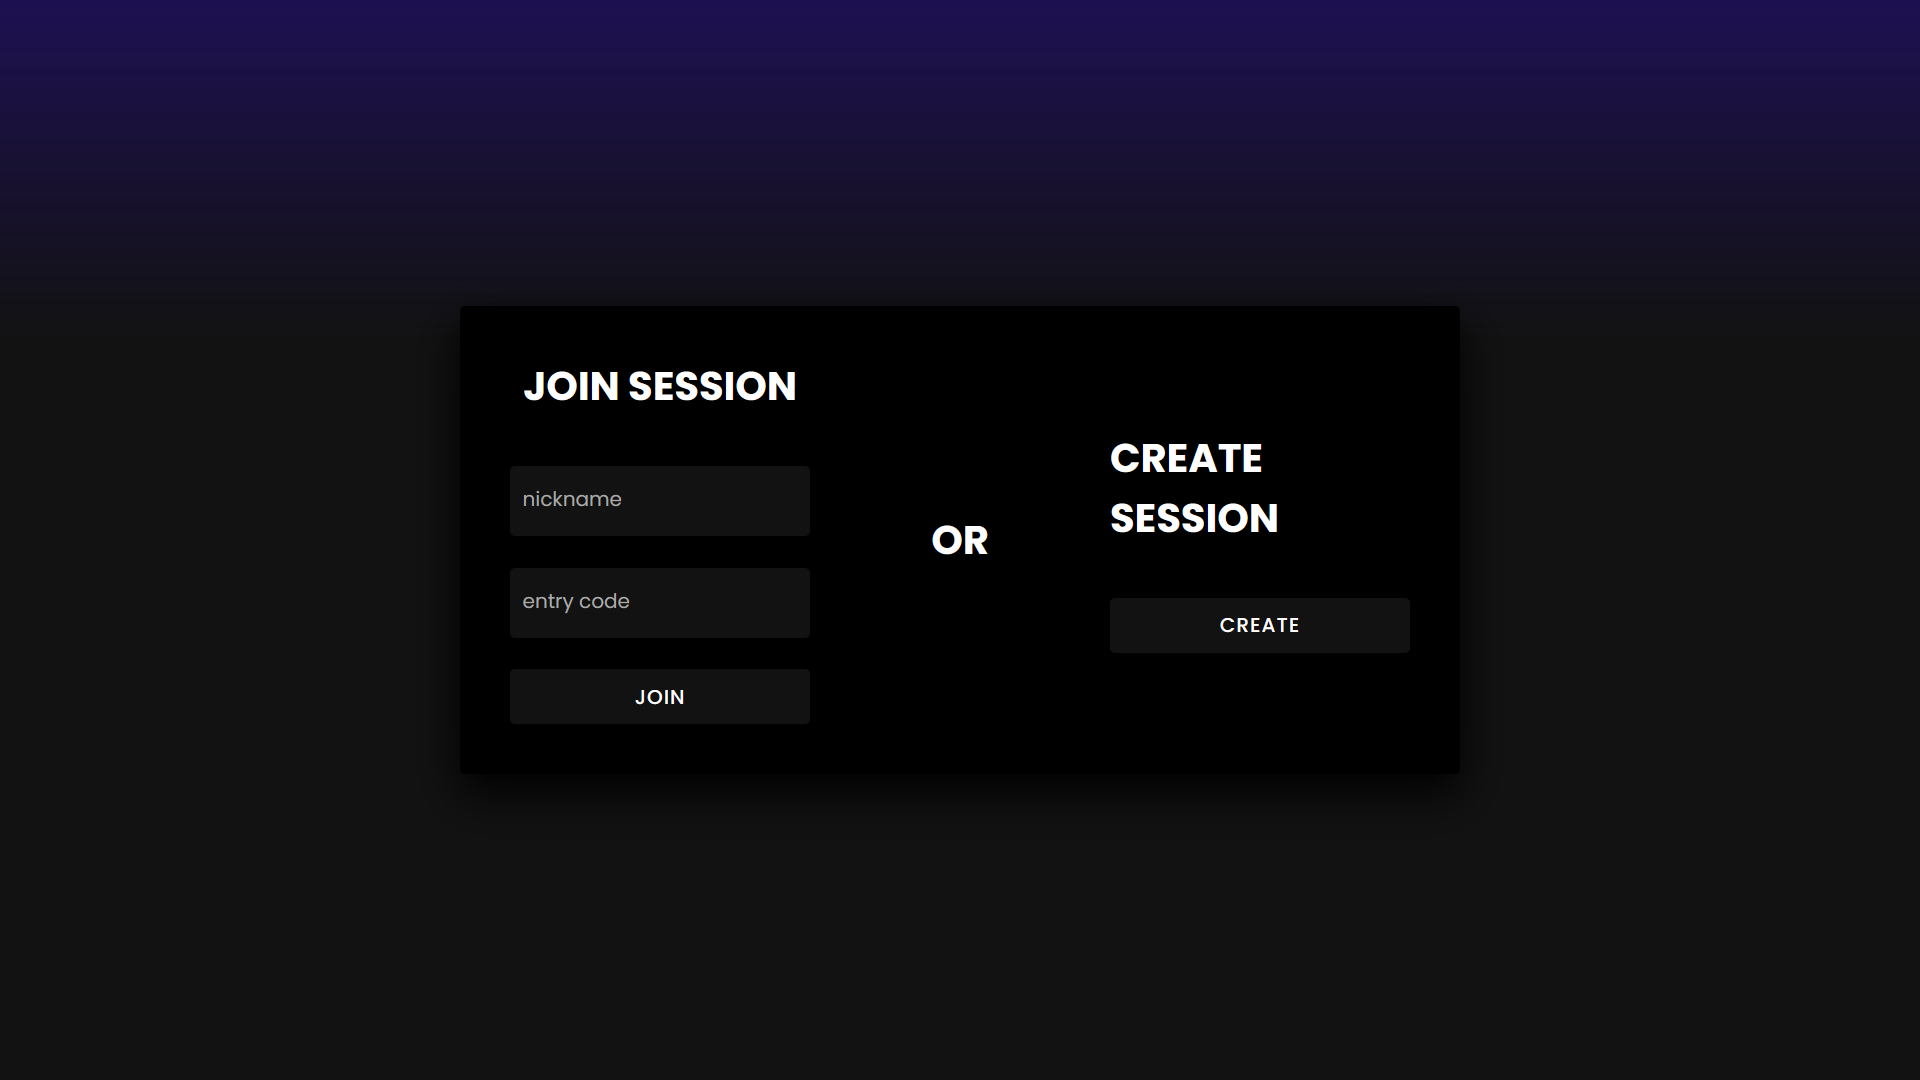
\includegraphics[width=0.95\textwidth]{./graf/auth_menu.png}
\caption{Wygląd interfejsu użytkownika - główne menu logowania}
\label{fig:auth-menu}
\end{figure}

\item Użytkownik jest przeniesiony na stronę autoryzacji Spotify, gdzie ma możliwość zalogowania się do swojego konta oraz proszony jest o wyrażenie zgody na określone warunki (Rys. \ref{fig:spotify-menu}).
\begin{figure}[h]
\centering
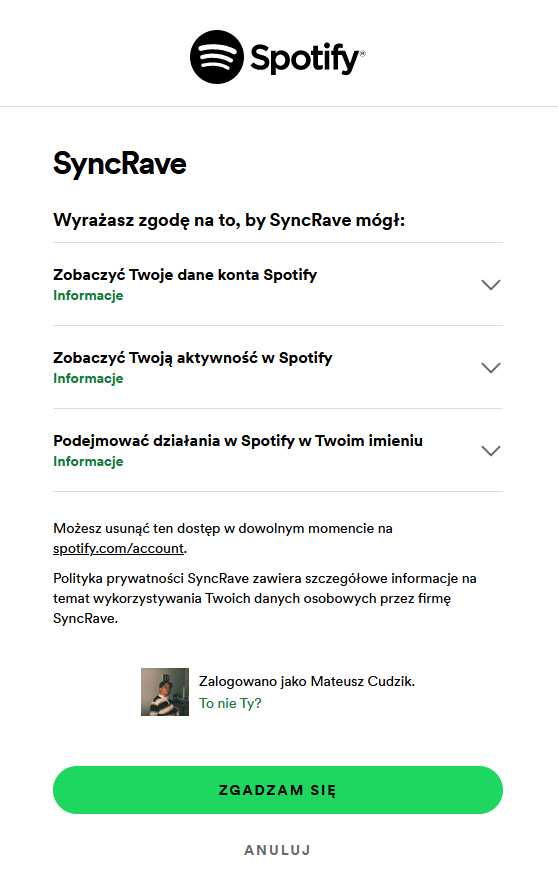
\includegraphics[width=0.95\textwidth]{./graf/spotify_permission.PNG}
\caption{Wygląd interfejsu użytkownika - menu wyrażenia zgody w serwisie Spotify}
\label{fig:spotify-menu}
\end{figure}

\item System przenosi użytkownika do menu gdzie udostępniony jest formularz zakładania sesji (Rys. \ref{fig:admin-menu}).
\begin{figure}[h]
\centering
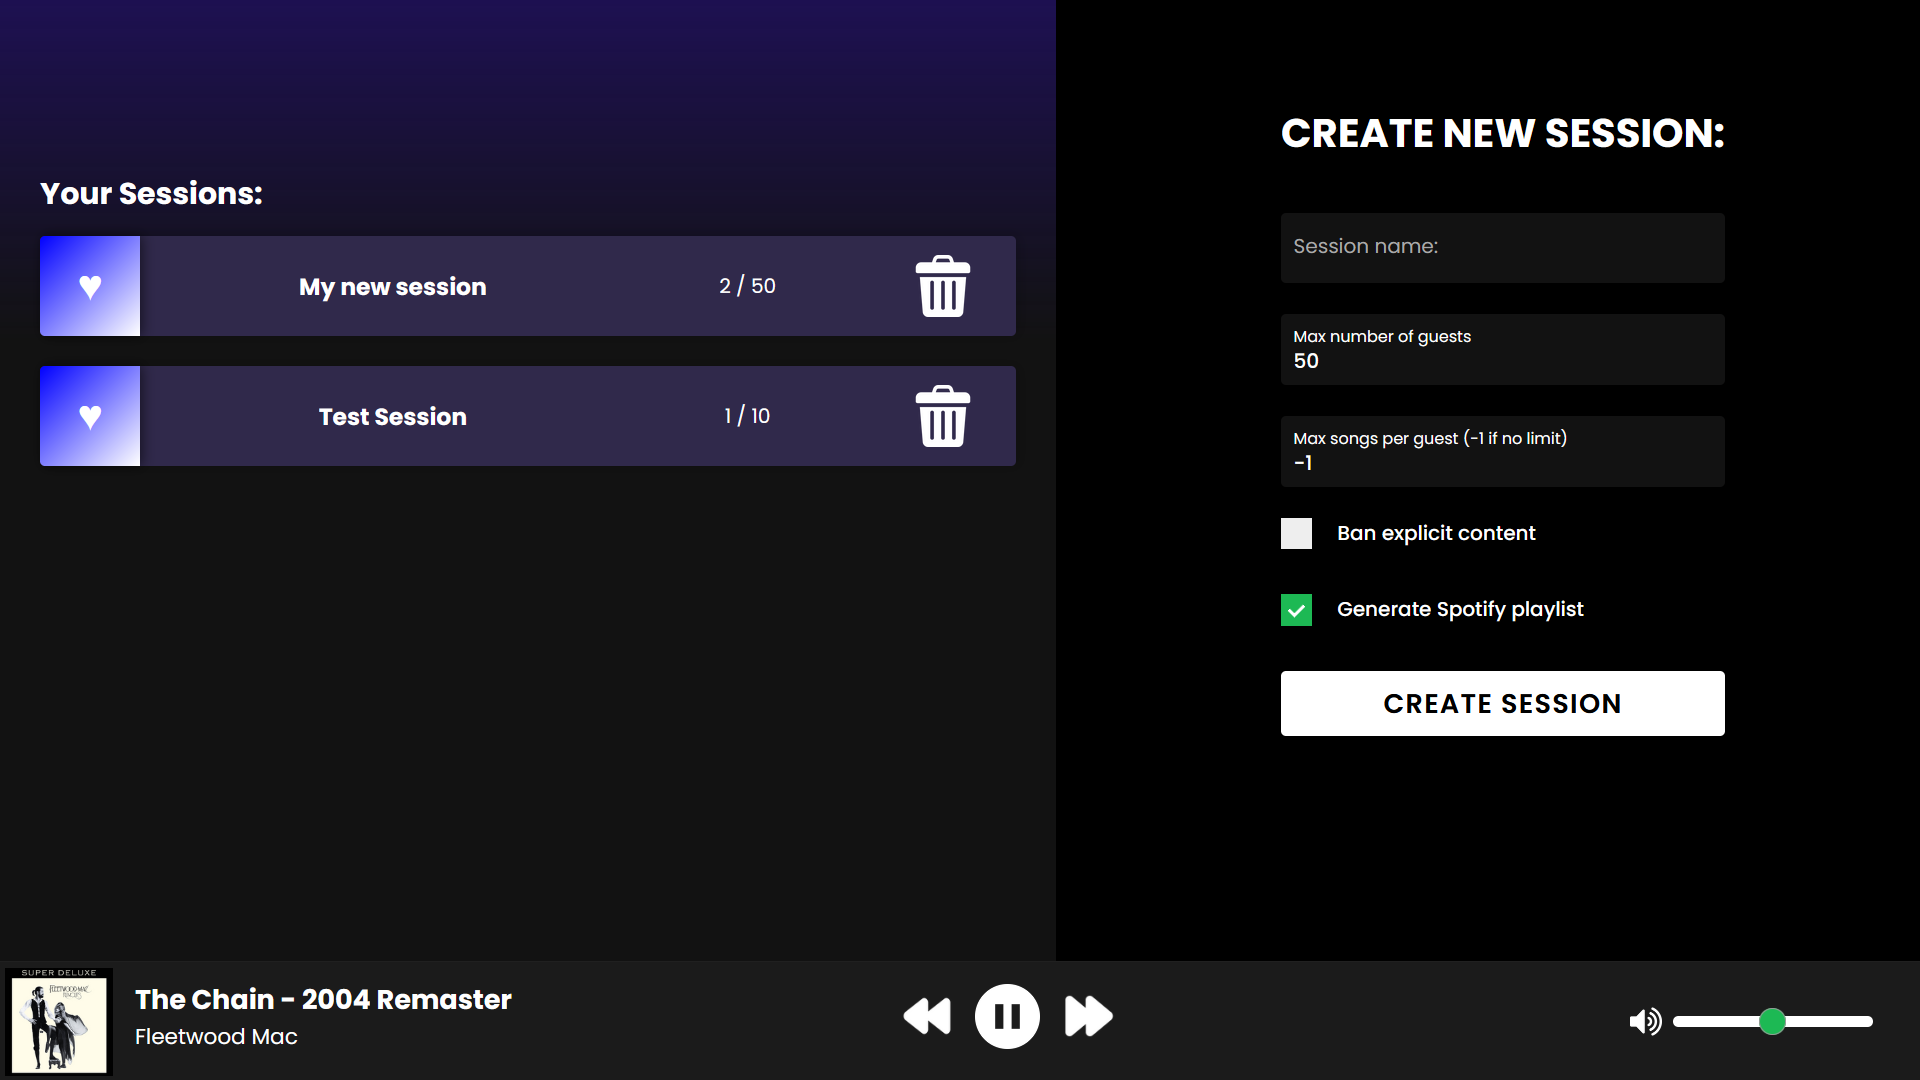
\includegraphics[width=0.95\textwidth]{./graf/admin_menu.png}
\caption{Wygląd interfejsu użytkownika - główne menu właściciela sesji}
\label{fig:admin-menu}
\end{figure}

\item Po wypełnieniu i zatwierdzeniu przez użytkownika formularza, system sprawdza poprawność wypełnionych danych.
\item Dodana sesja pojawia się z lewej strony menu właściciela sesji.
\item Jeśli użytkownik zdecyduje się dołączyć do jednej z sesji wybiera ją z listy.
\item System przenosi użytkownika do widoku sesji w wersji właściciela (Rys. \ref{fig:session-menu-owner}).
\begin{figure}[h]
\centering
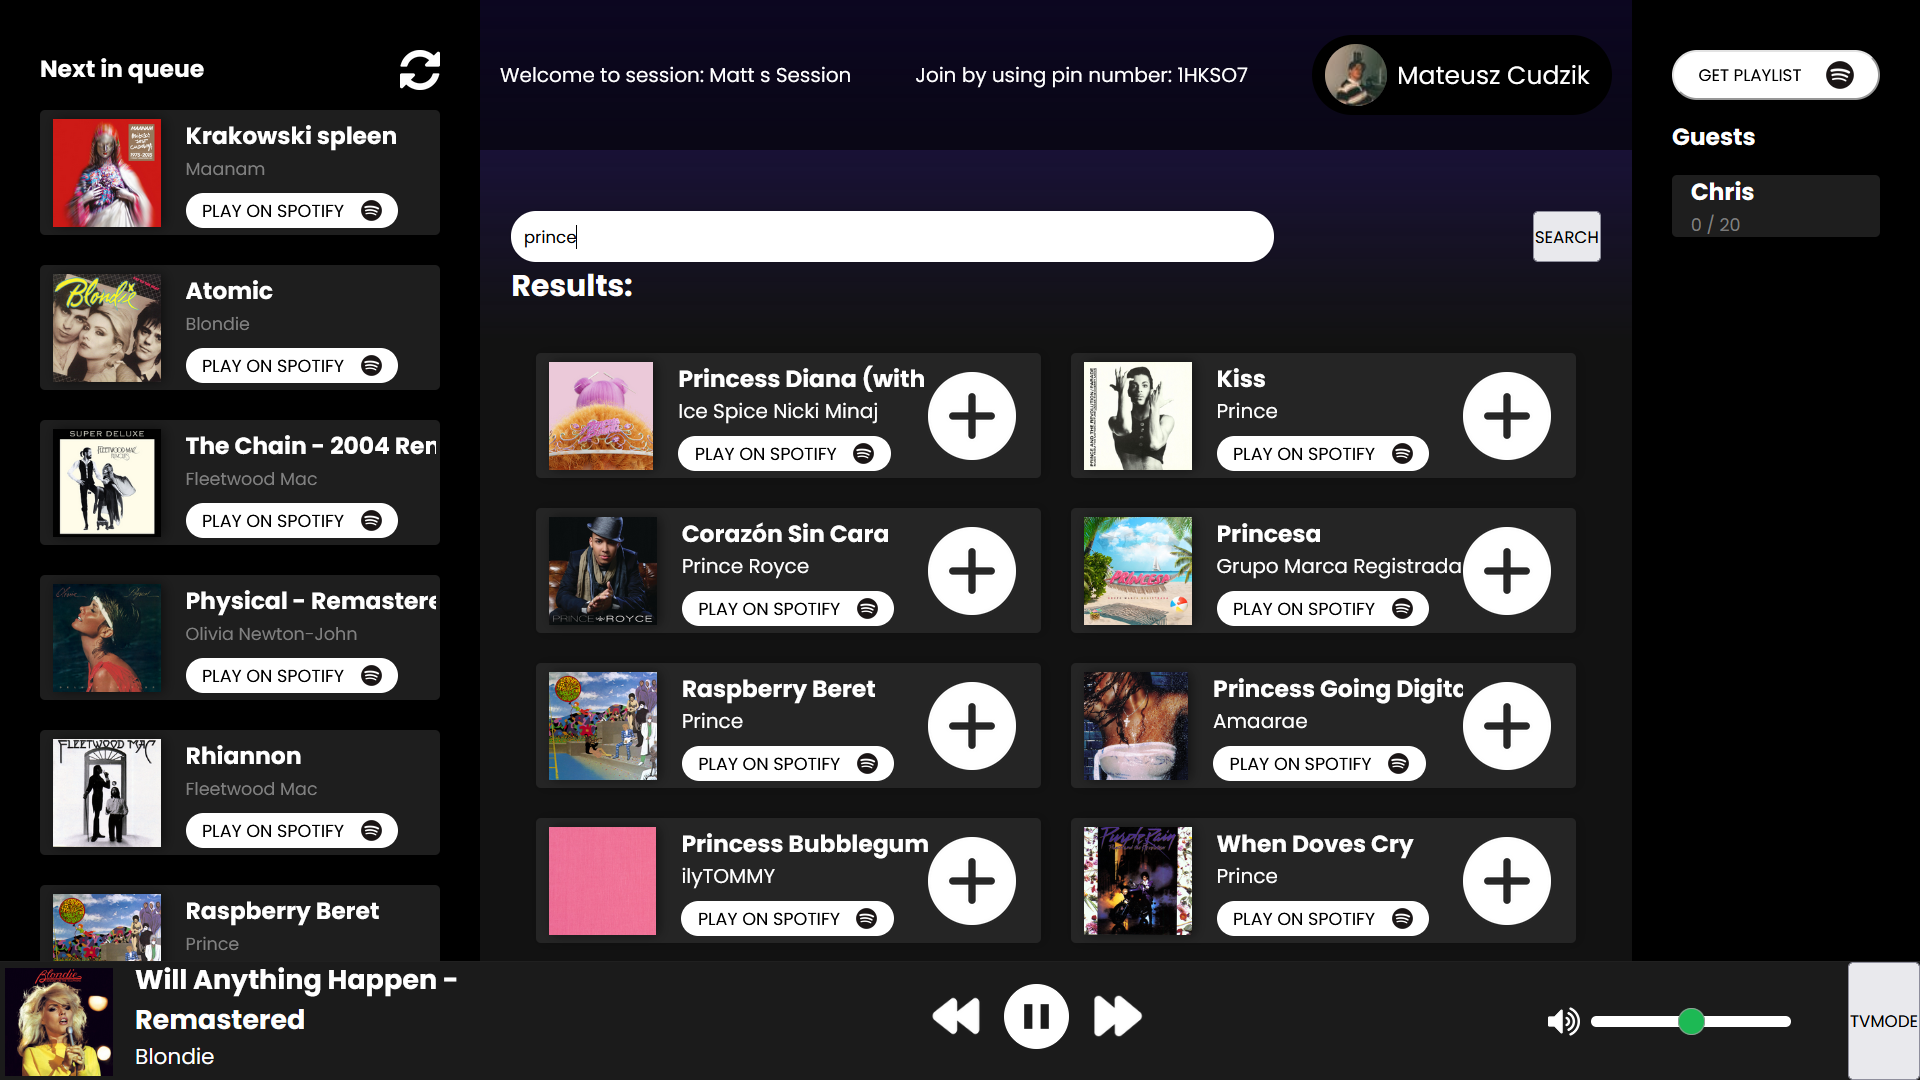
\includegraphics[width=0.95\textwidth]{./graf/admin_session_menu.png}
\caption{Wygląd interfejsu użytkownika - widok sesji w wersji właściciela}
\label{fig:session-menu-owner}
\end{figure}
\end{enumerate}

\subsection{Dołączenie do istniejącej sesji}
\begin{enumerate}
\item Przypadek rozpoczyna się, gdy użytkownik uruchomi aplikację w przeglądarce internetowej przez wpisanie poprawnego adresu lub zeskanowanie kodu QR z adresem.
\item System wyświetla użytkownikowi menu (Rys. \ref{fig:auth-menu}), w którym proszony jest o wpisanie pseudonimu, którym będzie się posługiwał oraz kodu dostępu do sesji. W przypadku gdy użytkownik zeskanował kod QR kod dostępu będzie automatycznie wpisany w odpowiednie pole.
\item Po zatwierdzeniu formularza system sprawdza poprawność danych.
\item Użytkownik przeniesiony jest do menu widoku sesji w wersji gościa (Rys. \ref{fig:session-menu-guest}). Przypadek użycia się kończy.
\begin{figure}[h]
\centering
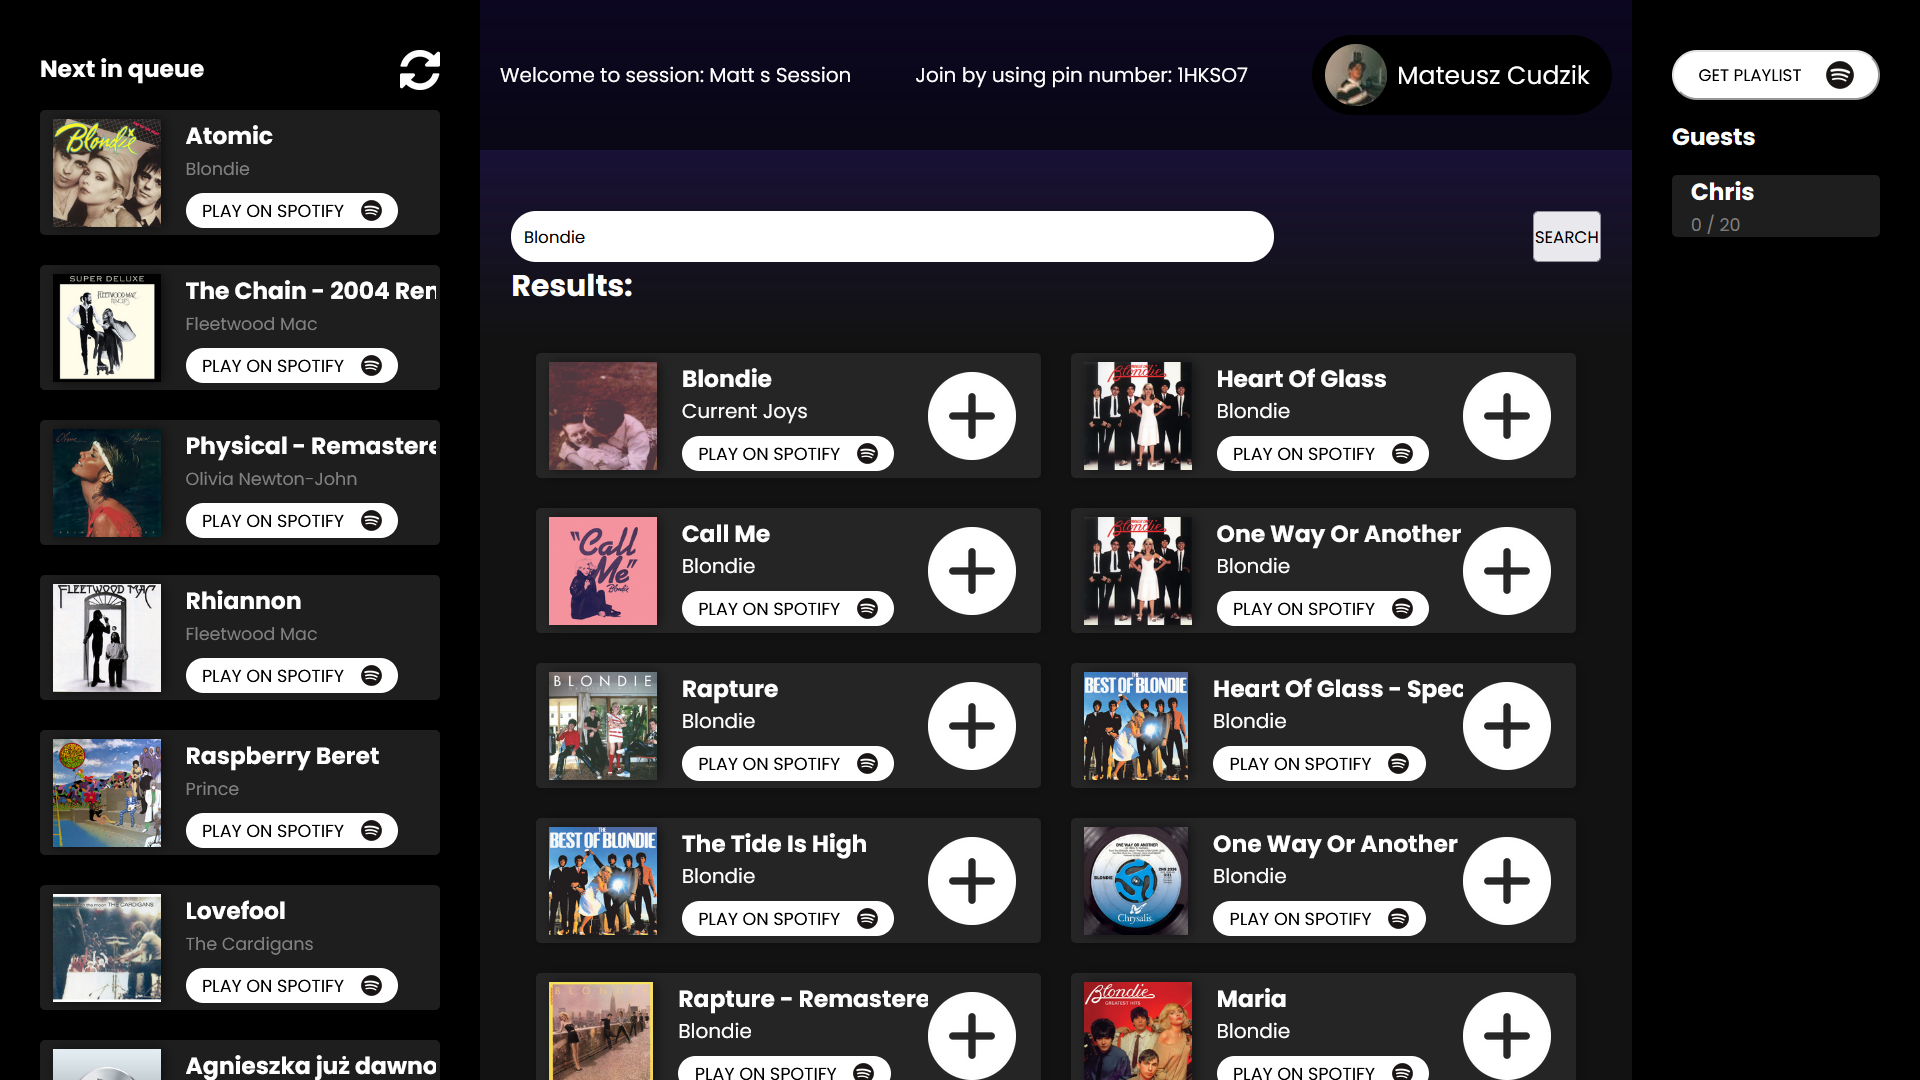
\includegraphics[width=0.95\textwidth]{./graf/guest_session_menu.PNG}
\caption{Wygląd interfejsu użytkownika - widok sesji w wersji gościa}
\label{fig:session-menu-guest}
\end{figure}
\end{enumerate}

\subsection{Dodawanie utworu do kolejki}
\begin{enumerate}
\item Przypadek rozpoczyna się gdy użytkownik znajduje się w menu widoku sesji Rys. \ref{fig:session-menu-guest} lub Rys. \ref{fig:session-menu-owner}.
\item Użytkownik wpisuje w pole wyszukiwania odpowiednią frazę. Może to być artysta, tytuł utworu lub albumu.
\item Po zatwierdzeniu system zwraca wyniki wyszukiwania.
\item Użytkownik może dodać znaleziony utwór używając odpowiedniego przycisku obok wyniku.
\item Jeśli utwór spełnia zasady sesji oraz użytkownik nie osiągnął limitu utwór zostaje dodany na koniec kolejki. Limity te nie dotyczą właściciela sesji. Przypadek użycia się kończy.
\end{enumerate}

